\documentclass[12pt,notitlepage]{report}

%\usepackage[cm]{fullpage}
\usepackage{amsmath}
\usepackage{fullpage}
\usepackage[nottoc]{tocbibind}
\usepackage{etoolbox}

%\usepackage{etoolbox}
%\makeatletter
%\patchcmd{\chapter}{\if@openright\cleardoublepage\else\clearpage\fi}{}{}{}
%\makeatother

%\setlength{\topmargin}{0.00in}
%\setlength{\textheight}{8.75in}
%\setlength{\textwidth}{6.625in}
%\setlength{\oddsidemargin}{0.0in}
%\setlength{\evensidemargin}{0.0in}

\begin{document}

\setcounter{tocdepth}{4}

\title{An Investigation into Heterogeneous CPU/GPGPU Computing}
\author{Kevin Dawkins\\
  Department of Computer Science,\\
  University of Arizona,\\
  Tucson, Arizona\\
  \texttt{kdawkins@cs.arizona.edu}}
\date{\today}
\maketitle

\null\vfill
\begin{abstract}
In this project I will investigate the shift in architectures occurring in the GPGPU (General Purpose GPU�s, as opposed to simple graphics GPUs) space. Current generation architectures place the GPGPUs over the PCI-e bus and move data from main memory to the GPGPU specific memory across the front side bus as necessary. However, a shift is occurring, and the next generation architectures (for example, Nvidia�s Tegra 5) are beginning to incorporate the GPGPUs into the main CPU complex itself.  This heterogeneous multicore architecture solves some problems such as the data movement across the PCIe bus, but creates its own set of challenges related to memory, timing and ISA design since the GPGPU runs much differently than the CPU. \\

This project will compare and contrast the advantages and disadvantages of multicore CPU systems with mixed CPU and GPGPU forms of computing, and investigate into the future architecture of the system in a heterogeneous multicore world. 
\end{abstract}


\tableofcontents

\chapter*{Introduction}
\addcontentsline{toc}{chapter}{Introduction}
A fundamental shift is occurring, beginning with the advent of the General Purpose Graphics Processing Unit (GPGPU) capable of much more processing than simply generating scenes for video games. This unit can handle specific workloads much more efficiently than a general CPU. While these workloads are specialized, in the increasingly parallel computing environments of today, it is finding much more use. However, it has been hampered by the large cost of moving massive amounts of data from the CPU onto the GPGPU's memory. To help bring the GPGPU to its fullest potential, it is getting swept into the CPU's increasing core count. Joining the general cores on the CPU itself. 

This shift comes with its own history spawning from GUI creators trying to solve their own unique problem to big data researchers realizing the similarities their problems have. As the GPU evolved, its creators were inadvertently (or perhaps, intentionally) created another general purpose processing unit that put the much more complicated CPU to shame on its own class of problems. 

This shift does not come without its own unique challenges. The GPGPU's single instruction multiple data (SIMD) class of computing differs wildly from the CPU's single instruction single data (SISD) class. This paper found that the differences can be classified into the following aspects: Control Flow, Memory Access, and Data Transfer. This paper will analyze all three differences, and analyze solutions to these problems. 



\chapter*{The GPGPU}
\addcontentsline{toc}{chapter}{The GPGPU}
\section*{What is a GPU?}
\addcontentsline{toc}{section}{What is a GPU?}

Graphics Processing Units (GPUs) gained popularity during the mid-1990s. As computers became more prevalent in consumers homes, multimedia functions (games, animations, GUIs) became more demanding on system resources. Looking for a solution, researchers noticed that the types of work being done to draw the screen was unique in that the data set could be broken up into smaller independent data sets. These smaller data sets then had the same operation applied on each one in parallel. The final result was the combination of each data set. 

This style of computation became known as \textbf{S}ingle \textbf{I}nstruction \textbf{M}ultiple \textbf{D}ata (SIMD). The key observation being that each individual operation could be one on each data set in parallel. However, the programability of these operations was limited, initially not extending past transformation and lighting (hardware T$\&L$). 

The evolution of the programmable GPU can be traced with the evolution of Direct3D (commonly known as Microsoft's DirectX). With each evolution in the API, more flexibility was added to the GPU itself. \ref{tab:gpuevolution}

As shown in Table 1, the amount of control a programmer had over the GPU grew with each new iteration of DirectX. In fact, by DirectX 10 with the advent of the unified shader, it was theoretically possible to use the GPU as a floating-point coprocessor. It was at this point, researches started to notice that other computational problems outside of drawing the screen would greatly benefit from the GPUs style of computation. This revelation would change GPU design, even changing its name to the \textbf{G}eneral \textbf{P}urpose graphics processing unit (GPGPU). \cite{emergingtech}

\begin{table}
	\begin{tabular}{|c|c|}
		\hline
		\textbf{DirextX Level} & \textbf{Programmability} \\
		\hline
		$<$ 8.0 & Nothing beyond advanced texture blending \\
		8.0 & Assembly language for vertex processing \\
		9.0 & Data dependent branching and fragment program assembly\\
		10.0 & Unified Vertex/Fragment shaders, Memory Scatter \\
		\hline
	\end{tabular}
	\caption{Evolution of programmable GPUs}
	\label{tab:gpuevolution}
\end{table}


\section*{The birth of the GPGPU}
\addcontentsline{toc}{section}{The birth of the GPGPU}

Unified shaders can be attributed to the single most important moment in the creation of a General Purpose GPU. The unified shader means that the vertex and fragment shaders were combined into one unit. Each GPU would have multiple unified shader units. These units adapted to the needs of the current data set, they could be used as either vertex or fragment shaders varying dynamically during execution. 

Unified shaders also provided one more important attribute to the birth of the GPGPU, a single language to control everything programmable on the GPU. Prior to this, programmers had to know about both the vertex shader language, and the fragment shader language. This was a huge burden to programmers not writing multimedia applications. Unifying the programming language also allowed people to start working on higher level languages for the GPGPU. \textbf{need to cite} 

Another advantage that the GPU had was its massive number of cores and possible concurrent threads. For programs that could take advantage of the SIMD architecture, could expect to run on a massive amount of hardware. For example, the NVIDIA Geforce 8 architecture, allowed programs to run on 128 processor cores and execute a dizzying 12,228 concurrent threads! GPUs could eclipse the CPU when comparing floating point operations by a huge scale. \cite{emergingtech}

The unified shader represented a more general approach to the CPU freeing programmers from writing their GPGPU programs using the terms of a graphics program. This created an opportunity for GPGPU hardware and programming models to be defined centered around general purpose programming. NVIDIA's Compute Unified Device Architecture (CUDA) was one of the first, allowing programmers to write in a C-like language. 

The ability to write programs in a C-like general language rather than a specialized shader language (that required the programmer to write everything in terms of graphics nomenclature, combined with the increasingly general aspects of the GPU meant that the industry could start porting applications and attempting to figure out what works well on a GPGPU. 

\section*{Unleashing the power of the GPGPU}
\addcontentsline{toc}{section}{Unleashing the power of the GPGPU}


Now that programmers had the tools and APIs they need, programs and experimentation was done to determine what worked well on the GPGPU. The following is a sample of real world applications ported to a GPGPU because of their access patterns and potential for performance gains. 

They will be briefly presented here, but the details regarding their porting and lessons learned about GPGPU architecture will not be discussed in detail here. Later in the paper, these topics will be fully discussed and these projects will be referenced. 

\subsection*{Linear Algebra}
\addcontentsline{toc}{subsection}{Linear Algebra}

Perhaps one of the most obvious general uses of a GPGPU lays in the realm of liner algebra. It seems fitting since the GPU was designed around matrix math (pixels on a screen). 

A Cholesky factorization is a common linear algebra operation run on a matrix. By breaking the matrix down into smaller chunks and running the factorization on them, the authors were able to achieve a 3.8X speedup over the standard Intel CPU math library. \cite{linearalg}

\subsection*{Big Data}
\addcontentsline{toc}{subsection}{Big Data}

** I would like to find one of these. But since the paper focuses on the arch, and I have the two others, I may not need it or it would be overkill. Both the memcached and linear papers focus on why the GPU arch is different. 

\subsection*{memcached}
\addcontentsline{toc}{subsection}{memcached}


Memcachd is a distributed memory object cache system. It was designed during the rising popularity of dynamic content on the internet. Memcached stores recently used database information in memory. All of the stored information is combined into massive hash tables. These tables must be crawled efficiently and quickly in order for a performance gain to be attained. The potential problem is that incoming requests are largely dependent on changing data. 

The GPGPU version of memcached ported the \textit{GET} command (after an observation that most requests are \textit{GET} and the write commands may fair better on the CPU. Requests are batched then ran in parallel on the GPGPU running the hash computation and lookup in parallel. Their findings showed that the GPGPU outperformed the CPU by factors reaching 7X speedup. \cite{memcached}


\subsection*{A move into the future}
\addcontentsline{roc}{subsection}{A move into the future}

Combining the ability to perform general purpose computing utilizing common programming languages, and results showing the real world use of GPGPUs the stage has been set for a big revolution in computing. However, if GPGPUs are ever expected to breach into enterprise workloads an integration must take place. All the results showed that while GPGPUs are great for their tasks, they are even better when working closely with the CPU. 

For this change to be meaningful, there must be an efficient line of communication for the CPU and the GPGPU to work together on tasks without a lot of overhead. The current generation of GPGPUs rely on an external bus to bridge the communication and data between the CPU and GPGPU (commonly the PCI-e bus). With data sets growing larger, this is becoming a huge bottleneck that can slow the rest of the system and causes one to constantly wait on the other.

Enter the world of heterogenous computing. Combining a GPGPU directly into the cores of the CPU itself. This has the chance to dramatically increase performance allowing almost seamless transfer whenever appropriate. This does not come without its challenges, and the rest of the paper will explore these in detail, proposing solutions along the way. 














\chapter*{How is the GPGPU different?}
\addcontentsline{toc}{chapter}{How is the GPGPU different?}
\subsection*{Architecture Differences}
\addcontentsline{toc}{section}{Architecture Differences}

Talking about the hardware. Stream processors VS general purpose CPU cores also talk about SIMD

\subsection*{How does a GPGPU process data?}
\addcontentsline{toc}{section}{How does a GPGPU process data?}

As discussed in the previous section, GPGPUs utilize the Single Instruction Multiple Data (SIMD) architecture. In this architecture, all executing threads must move through the computation in lock-step. Threads cannot deviate from the execution path. Ideally threads would execute without branches or control flow operations that would effect their route through the GPGPU. The efficiency of a GPGPU (SIMD efficiency) is defined as "the fraction of scalar threads that execute together in lockstep per cycle" \cite{memcached}

GPGPU architecture varies from a general purpose CPU architecture in three main ways, Control Flow, Memory Access, and Data Transfer. These all end up as challenges when incorporating the GPGPU into the CPU to create the heterogeneous architecture. 

\subsection*{Control Flow}
\addcontentsline{toc}{subsection}{Control Flow}

Recall that in a SIMD (Single Instruction Multiple Data) architecture, all concurrently executing threads (also known as workgroups) must move through the GPPGU in lock-step. Therefore, the ideal situation for these wavefronts would be to move through the code with no conditional branches allowing unabated forward progress through the program and correctly executing instructions for each work item (data set) in parallel. 

However, this is almost never the case. Modern mature programs almost always include control flow branches in the code. With that being said, it is entirely possible for threads in the wavefront to encounter data items that cause the code to make the jump, while the rest of the threads do not. Predictably, this causes problems when threads are expected to execute in lock step. This is known as "branch divergence" and is currently solved with the addition of a hardware component that monitors the running threads. This SIMT stack monitor watches threads executing and disables threads making an uncharacteristic jump. It tracks the current program counter and the RPC (re-convergance program counter), which is the closest point in the code at which the inactive and active threads will rejoin. 

This does not cause the threads that made the jump to miss out on any execution. As soon as the active threads finish executing their code the converge and the inactive threads continue execution. The main difference here is that on a CPU, if threads on executing on different cores diverge, they can all continue execution on their own paths. Each core can be at a vastly different place in the program but still actively executing code. However, the GPGPU runs like a train, and must sequentially walk through the entire program, so divergent threads, rather than executing in different places, inactivate for the points in the code they do not execute. 

\chapter*{Merging the CPU with a GPGPU}
\addcontentsline{toc}{chapter}{Merging the CPU with a GPGPU}
\section*{The Motivation Behind the Merge}
\addcontentsline{toc}{section}{The Motivation Behind the Merge}

This massively complex initiative to move the GPGPU onto the CPUs cores will provide huge advantages to programmers and computer designers in the future. These advantages in design and implementation result in more efficient programs, and an attempt at helping with the power wall. Briefly, the power wall is a result of performance scaling faster than power dissipation has. Simply put, faster computers are more difficult to keep cool.  

One of the big power draws in the system is the GPGPU sitting on the PCI-e bus. These huge cards draw a lot of power, and create a lot of heat. Besides powering (and cooling) the GPGPU core itself, the cards must cool the supplementary memory that the cards contain. Most of this energy spent on cooling the GPGPU will be alleviated by merging it onto the CPU. It can share the DRAM and cache with the CPU taking its own hot memory out of the equation. 

In addition to cooling the cards, the processor spends a lot of energy and time transporting all of the data the cards need. This can cause huge delays on the pipeline and tie up crucial buses. Moving the GPGPU onto the CPU can eliminate the time spent moving this data around. As mentioned previously, the GPGPU would share the memory infrastructure with the CPU allowing it easy access to any data it needs. 

Finally, the merge could bring great benefits to the programmer. Currently, while writing a program using CUDA or Open CL, the programmer must navigate an awkward interface to determine which parts of the program must be run on the GPGPU and reference the device (and track the reference) throughout the code. Hopefully, in a heterogeneous environment, the programmer could utilize a GPGPU with little or no effort. This could either be accomplished by the compiler, or through a process as painless as standard C pthreads. 

\section*{The Status Quo}
\addcontentsline{toc}{section}{The Status Quo}

Work has already begun in the space. Intel's Sandy Bridge architecture moved the GPGPU form the north-bridge onto the CPU chip itself.\cite{tlpcache} This may have been for either cost saving reasons or for performance, but this represented a step in the march towards a heterogeneous architecture. Their fusion placed the GPGPU onto the die sharing a L3 cache and main memory. It however, is not, integrated into the CPU itself (as a heterogeneous architecture would be). Therefore, while the GPGPU and CPU have been integrated into the same chip, the programmer still writes code in the same way as before. In this model, the CPU will act as leader sending instructions, data, and code down to the GPGPU. 

Even still, this move is interesting because it pronounces some of the architecture questions around the integration between the CPU and the GPGPU. For one, how is the instruction set going to change? Will the CPU act as a leader dispatching instructions or will the compiler need to generate code specifically for the GPGPU core? For a completely efficient and effective heterogeneous architecture, the CPU cannot be expected to constantly lead the GPGPUs operations. That would force a bottleneck onto the CPU and require additional work on the CPU to determine what to send to the GPGPU. 


\section*{Writing Programs for a Heterogenous Enviornment}
\addcontentsline{toc}{section}{Writing Programs for a Heterogenous Enviornment}

When the GPGPU merges with the CPU, two distinct classes of programs will be written to take advantage of this new hardware both requiring different resources and interaction from the system. The first classification of program will utilize only the GPGPU without any need for the CPU. The other classification encompasses more complicated programs that utilize both the CPU and the GPGPU interchangeably throughout the programs execution. 

The first class of programs will require only cooperation from the operating system scheduler and the compiler. When this program type is built, the compiler will generate machine code only for the specific GPGPU target, without including any code for the CPU. This program will then be scheduled by the operating system to run on the GPGPU itself. 

The second class of program is more complicated. This will require a lightweight solution allowing the CPU to understand when instructions are meant for the GPGPU. The compiler will also have a role to play as it will need to target two different architectures at once! It will need to be able to generate machine code for both the CPU and the GPGPU and know when in the program the code need to be generated. While this compiler problem can be solved with flags, it is not in the scope of this paper. However, the instruction set for the CPU will need to be designed around the flexibility of accommodating both types of machine code interchangeably. 


\section*{Designing a \textit{Heterogenous} Instruction Set}
\addcontentsline{toc}{section}{Designing a \textit{Heterogenous} Instruction Set}

In order for efficient operation on par with a CPU, the GPGPU will need to be able to accept instructions during execution outside of the control of the CPU. To accomplish this without increasing the complexity and logic behind the CPU's pipeline too much, the VLIW instruction style provides an interesting comparison to draw inspiration from. 

VLIW tried to take advantage of instruction level parallelism (ILP) by combining several instructions into one super instruction. The VLIW instruction would then be broken apart in the pipeline and each individual instruction executed in parallel. 

In the spirit of VLIW, the heterogenous instruction set would consist of one CPU instruction paired with one GPGPU instruction. This instruction would be processed by the CPU in its initial instruction decode stage, then passed onto the GPGPU through a bus. Much like the VLIW instructions, the heterogenous instructions could be passed without either the CPU or GPGPU instruction if there were none at that cycle. Since the GPGPU can take one instruction and pass it to all of its threads, it is not necessary to try to overload the long word instruction with multiple GPGPU entries.

However, in many cases the instructions may not sync up. The GPGPU pipeline is much deeper and not designed around the fast clock of the CPU. This situation would also be fine because the GPGPU can continue to accept instructions in the current wavefront, and the CPU can continue to run. The CPU would only stall if it needed the result of a GPGPU operation, as this is also the case in current configurations, it would not impact the program any more negatively than it presently does. This also follows the spirit of a heterogenous architecture treating the GPGPU like another one of the CPU's independent cores. 

However, obvious problems in efficiency stem from each GPGPU instruction being forced to pass through the CPU. 

\begin{figure}[h]
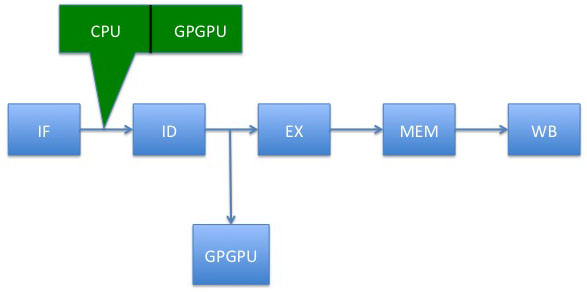
\includegraphics[scale=0.75]{diagrams/diag1.jpg}
\caption{Illustration of the heterogenous pipeline}
\end{figure}


\section*{Arbitration with the GPGPU}
\addcontentsline{toc}{section}{Arbitration with the GPGPU}

At first glance, it seems that the GPGPU should be treated like a peripheral component that can be locked down by running threads. However, that is not truly designing a heterogenous architecture. The best way to manage this different component would be to think of it as an additional CPU and give that problem to the operating system. As the different classes of programs were outlined previously, giving the operating system arbitration control over the GPGPU does not seem that challenging. The operating system would need to know when processes require the CPU vs. the GPGPU. 











\chapter*{Conclusion}
\addcontentsline{toc}{chapter}{Conclusion}
The General Purpose Graphics Processing Unit is becoming increasingly more relevant now that disciplines outside of games and multimedia are finding classes of problems that it can efficiently solve. However, as GPGPUs are currently being used as an additional component to the computer, they are contributing to the power wall which is slowing performance innovation. Also, as the classes of problems that GPGPUs can solve grows, so does the amount of data that they process. Transferring all of that data to an external card was proving to be a bottleneck on its own. 

Integrating GPGPUs into the CPU itself was the first step in trying to solve this problem. This presented its own class of challenges and opportunities for the programmer and system architect. This also started to alleviate stress on the power wall by allowing the GPGPU to utilize the memory of the CPU and the cooling infrastructure. However problems still existed as the GPGPU was being treated as a second class chip when compared to the CPU. It still was controlled and was issued instructions from the CPU. Also, data was being transferred to the GPGPU over a bus tying up the CPU.

As GPGPUs move into the future, heterogenous architectures are starting be created. This means that the GPGPU is directly included as a core on the CPU itself. Allowing the GPGPU to be accessed and run on its own provides challenges to systems architects. This paper identified two classes of GPGPU programs that could be run. The first was a stand alone program that had no interaction from the CPU. The second represented a more complicated GPGPU/CPU mixed program. These will typically be more common. The paper then identified solutions to these problems. 

The first case was solved with compiler and operating systems extensions supporting the GPGPU as an independently addressable core. The second more common case involved an instruction set modification allowing the program to pass both GPGPU instructions with CPU instructions. This allows the GPGPU to run without the program itself initiating the work, as a true additional core. 

With the growing popularity of the GPGPU, the ideal future would have it working invisibly to the programmer, as a component of the system that is used when needed, and suspended when not. This would greatly increase the capacity of the modern computer and the scope of work that it can efficiently compute. 

\nocite{nvidia, mapreduce, cpuassist}

\bibliography{paper}
\bibliographystyle{IEEEtran}


\end{document}